\documentclass{article}
\usepackage[letterpaper,top=0.5in,bottom=0.5in,left=1.2in,right=1.2in,includeheadfoot]{geometry}
\usepackage{amssymb,amsmath}
\usepackage{parskip}
\usepackage{fancyhdr}
\usepackage{enumerate}
\usepackage{enumitem}
\usepackage{graphicx}
\usepackage{xcolor}
\usepackage{listings}
\usepackage{float}
\usepackage[colorlinks=true,urlcolor=blue]{hyperref}

\lstset{
  basicstyle=\ttfamily\small,
  backgroundcolor=\color{gray!10},
  frame=single,
  breaklines=true,
  columns=fullflexible
}
 
\renewcommand{\baselinestretch}{1.3}
\pagestyle{fancy}
\fancyfoot{}
\renewcommand{\headrulewidth}{0pt}
\setlength{\headheight}{12pt}
\addtolength{\topmargin}{-12pt}
 
\fancypagestyle{firstpage}{
  \fancyhead{}
  \fancyfoot{}
}
 
\newcommand{\HomeworkNo}{5}
\newcommand{\MyName}{Julia Susser, Mudit Marwaha, Dhruv Bhargava}
 
\fancyhead[L]{\MyName}
\fancyhead[R]{Homework \HomeworkNo{}}
 
\newcommand{\PrintFirstHeader}{
\noindent NETS 1500 HW \HomeworkNo{} \hfill {\Large{\MyName}}

\vspace{3pt}
{\LARGE User Manual: The Reviewer Network}

\vspace{3pt}
\rule{\textwidth}{0.4pt}
\vspace{-30pt}
}
 
\begin{document}
\thispagestyle{firstpage}
\PrintFirstHeader{}
\allowdisplaybreaks

\subsection*{Project Overview}

We created a Java desktop application that analyzes the Amazon Fine Foods dataset (Stanford SNAP, 568,000 reviews). The concepts from class we used include graphs, recommender systems, document retrieval, and social networks.

TF-IDF Search allows you to enter a free-text query (e.g.\ ``organic coffee'') and receive a ranked list of matching products based on cosine similarity over review text.\\
Personalized PageRank Recommender allows you to enter a reviewer's user ID and receive a ranked list of products they have not yet reviewed, discovered via graph propagation from their highest-rated items.

\subsection*{Dataset}

This application uses the Amazon Fine Foods Reviews dataset from Stanford SNAP, containing $\sim$568,454 reviews, $\sim$256,059 users, and $\sim$74,258 products. The data is stored in plain-text key-value blocks, one review per block.
Source: \url{https://snap.stanford.edu/data/web-FineFoods.html}

Each review contains the following data fields:

\begin{center}
\begin{tabular}{lll}
\hline
Field & Description & Example \\
\hline
\texttt{productId}   & Unique product identifier        & B001E4KFG0 \\
\texttt{userId}      & Unique reviewer identifier       & A3SGXH7AUHU8GW \\
\texttt{profileName} & Reviewer's display name          & delmartian \\
\texttt{helpfulness} & Helpful votes / Total votes      & 1/1 \\
\texttt{score}       & Rating (1--5 stars)              & 5.0 \\
\texttt{time}        & Unix timestamp                   & 1303862400 \\
\texttt{summary}     & Short review title               & ``Good Quality Dog Food'' \\
\texttt{text}        & Full review text                 & ``I have bought several\ldots'' \\
\hline
\end{tabular}
\end{center}

\subsection*{Compiling the Program}

Run the following command to compile all files.

\begin{lstlisting}
javac -d out src/data/*.java src/util/*.java src/graph/*.java \
  src/analysis/*.java src/recommendation/*.java \
  src/app/*.java src/Main.java
\end{lstlisting}

Compiled \texttt{.class} files will be placed in the \texttt{out/} directory.

\subsection*{Running the Program}

\begin{lstlisting}
java -cp out Main
\end{lstlisting}
Add a custom data path: java -cp out Main --data input/finefoods.txt 

\subsection*{Application Window}

The application take a few seconds to load while the program parses reviews, builds the graph, and computes TF-IDF vectors. The status bar at the bottom always shows the number of nodes, edges, and reviews currently loaded.

\begin{figure}[H]
  \centering
    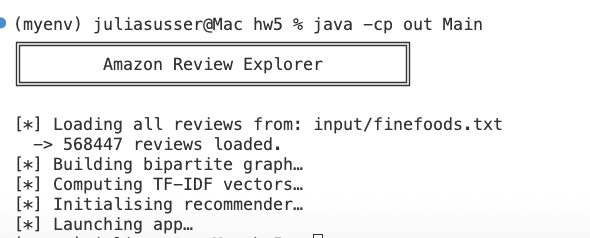
\includegraphics[width=0.9\textwidth]{imgs/launch.png}
  \caption{TF-IDF Search tab with results for the query ``organic coffee''.}
\end{figure}

\subsection*{Tab 1: TF-IDF Search}
This tab allows you to search for food products by entering a free-text query.
Type a query into the search bar at the top (e.g.\ ``organic green tea'', ``gluten free crackers'', ``dog food chicken'').\\
The results table populates with the top 20 matching products, ranked by TF-IDF cosine similarity score.\\
The results table columns are: rank (1 = most relevant), Product ID (the Amazon product identifier), Review Summary (the most representative review title for that product), and TF-IDF Score (cosine similarity between your query and the product's aggregated review text, where higher means more relevant).\\

\begin{figure}[H]
  \centering
    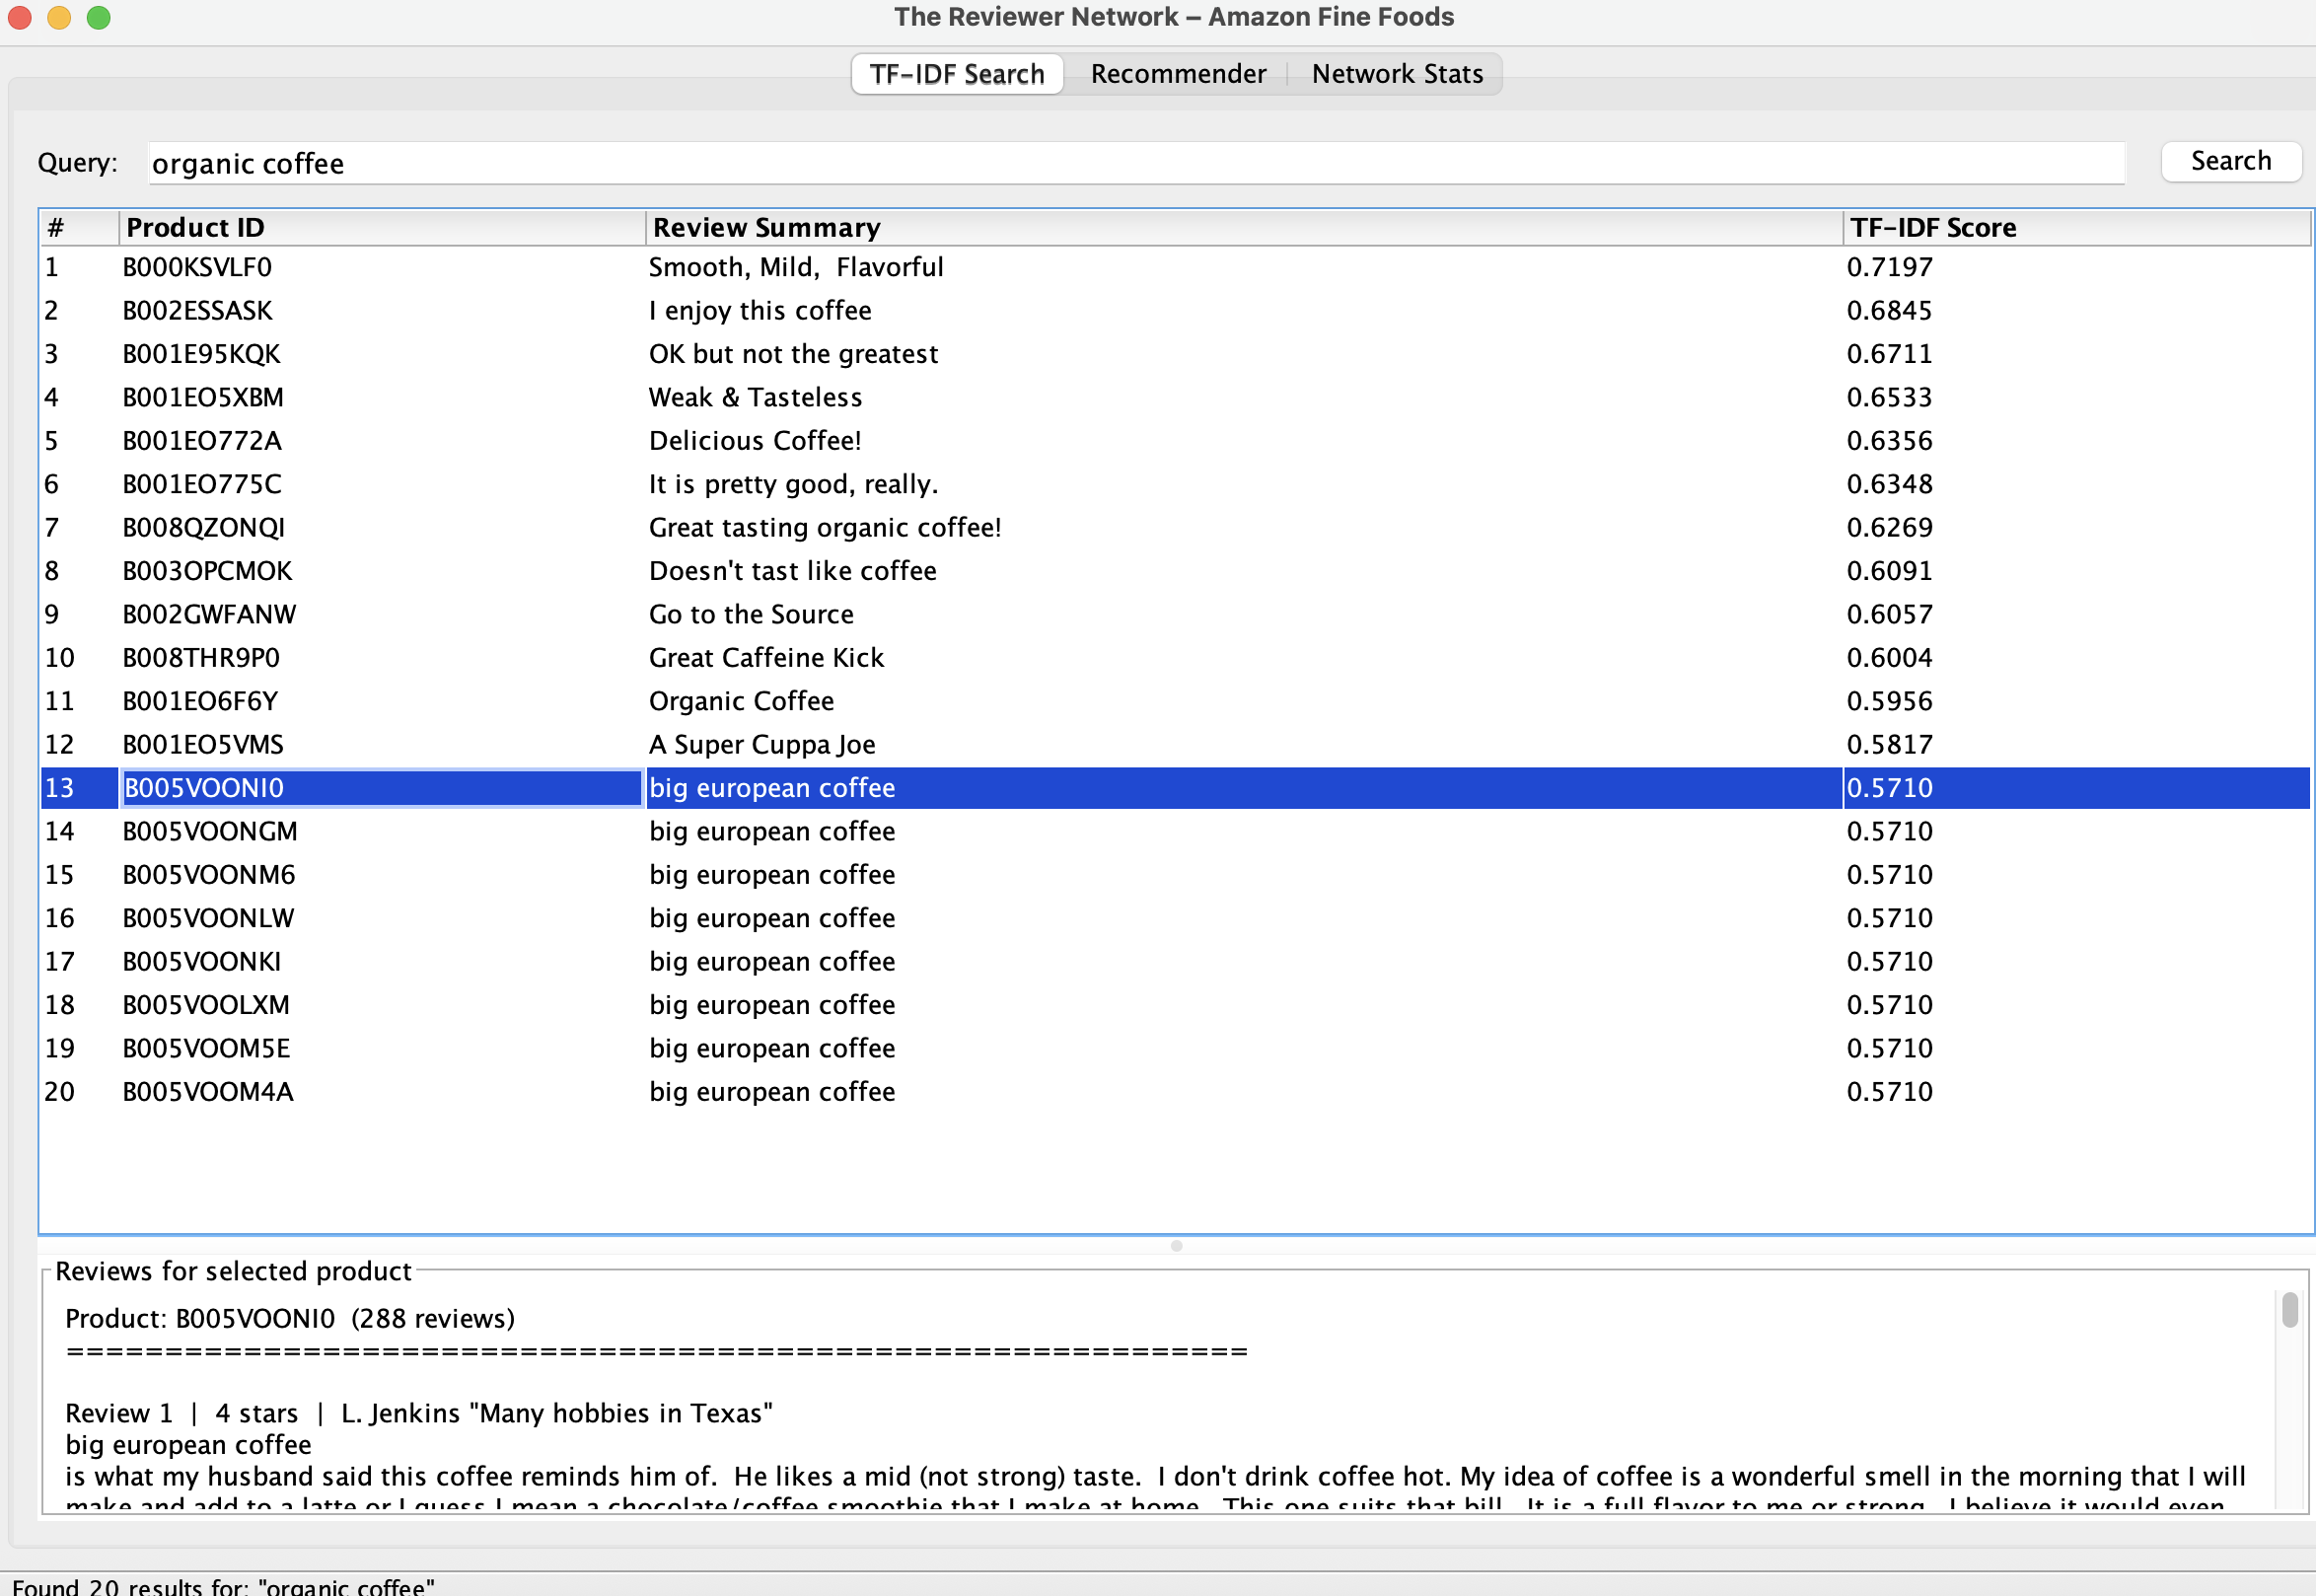
\includegraphics[width=0.9\textwidth]{imgs/tdif-search-results.png}
  \caption{TF-IDF Search tab with results for the query ``organic coffee''.}
\end{figure}

\subsection*{Tab 2: Recommender}
This tab provides personalized product recommendations for a specific reviewer using Personalized PageRank.\\
Enter a reviewer's User ID into the text field (e.g.\ \texttt{A3SGXH7AUHU8GW}) or click Random User to automatically select a reviewer with at least 3 reviews and run recommendations immediately.\\
The results table shows the top 20 products the user has not yet reviewed, ranked by their Personalized PageRank score.\\
The results table columns are: rank (1 = most recommended), Product ID (the Amazon product identifier), Review Summary (representative review title for that product), and PPR Score (Personalized PageRank score, where higher values indicate the product is more reachable from the user's highly-rated items in the graph).

\begin{figure}[H]
  \centering
  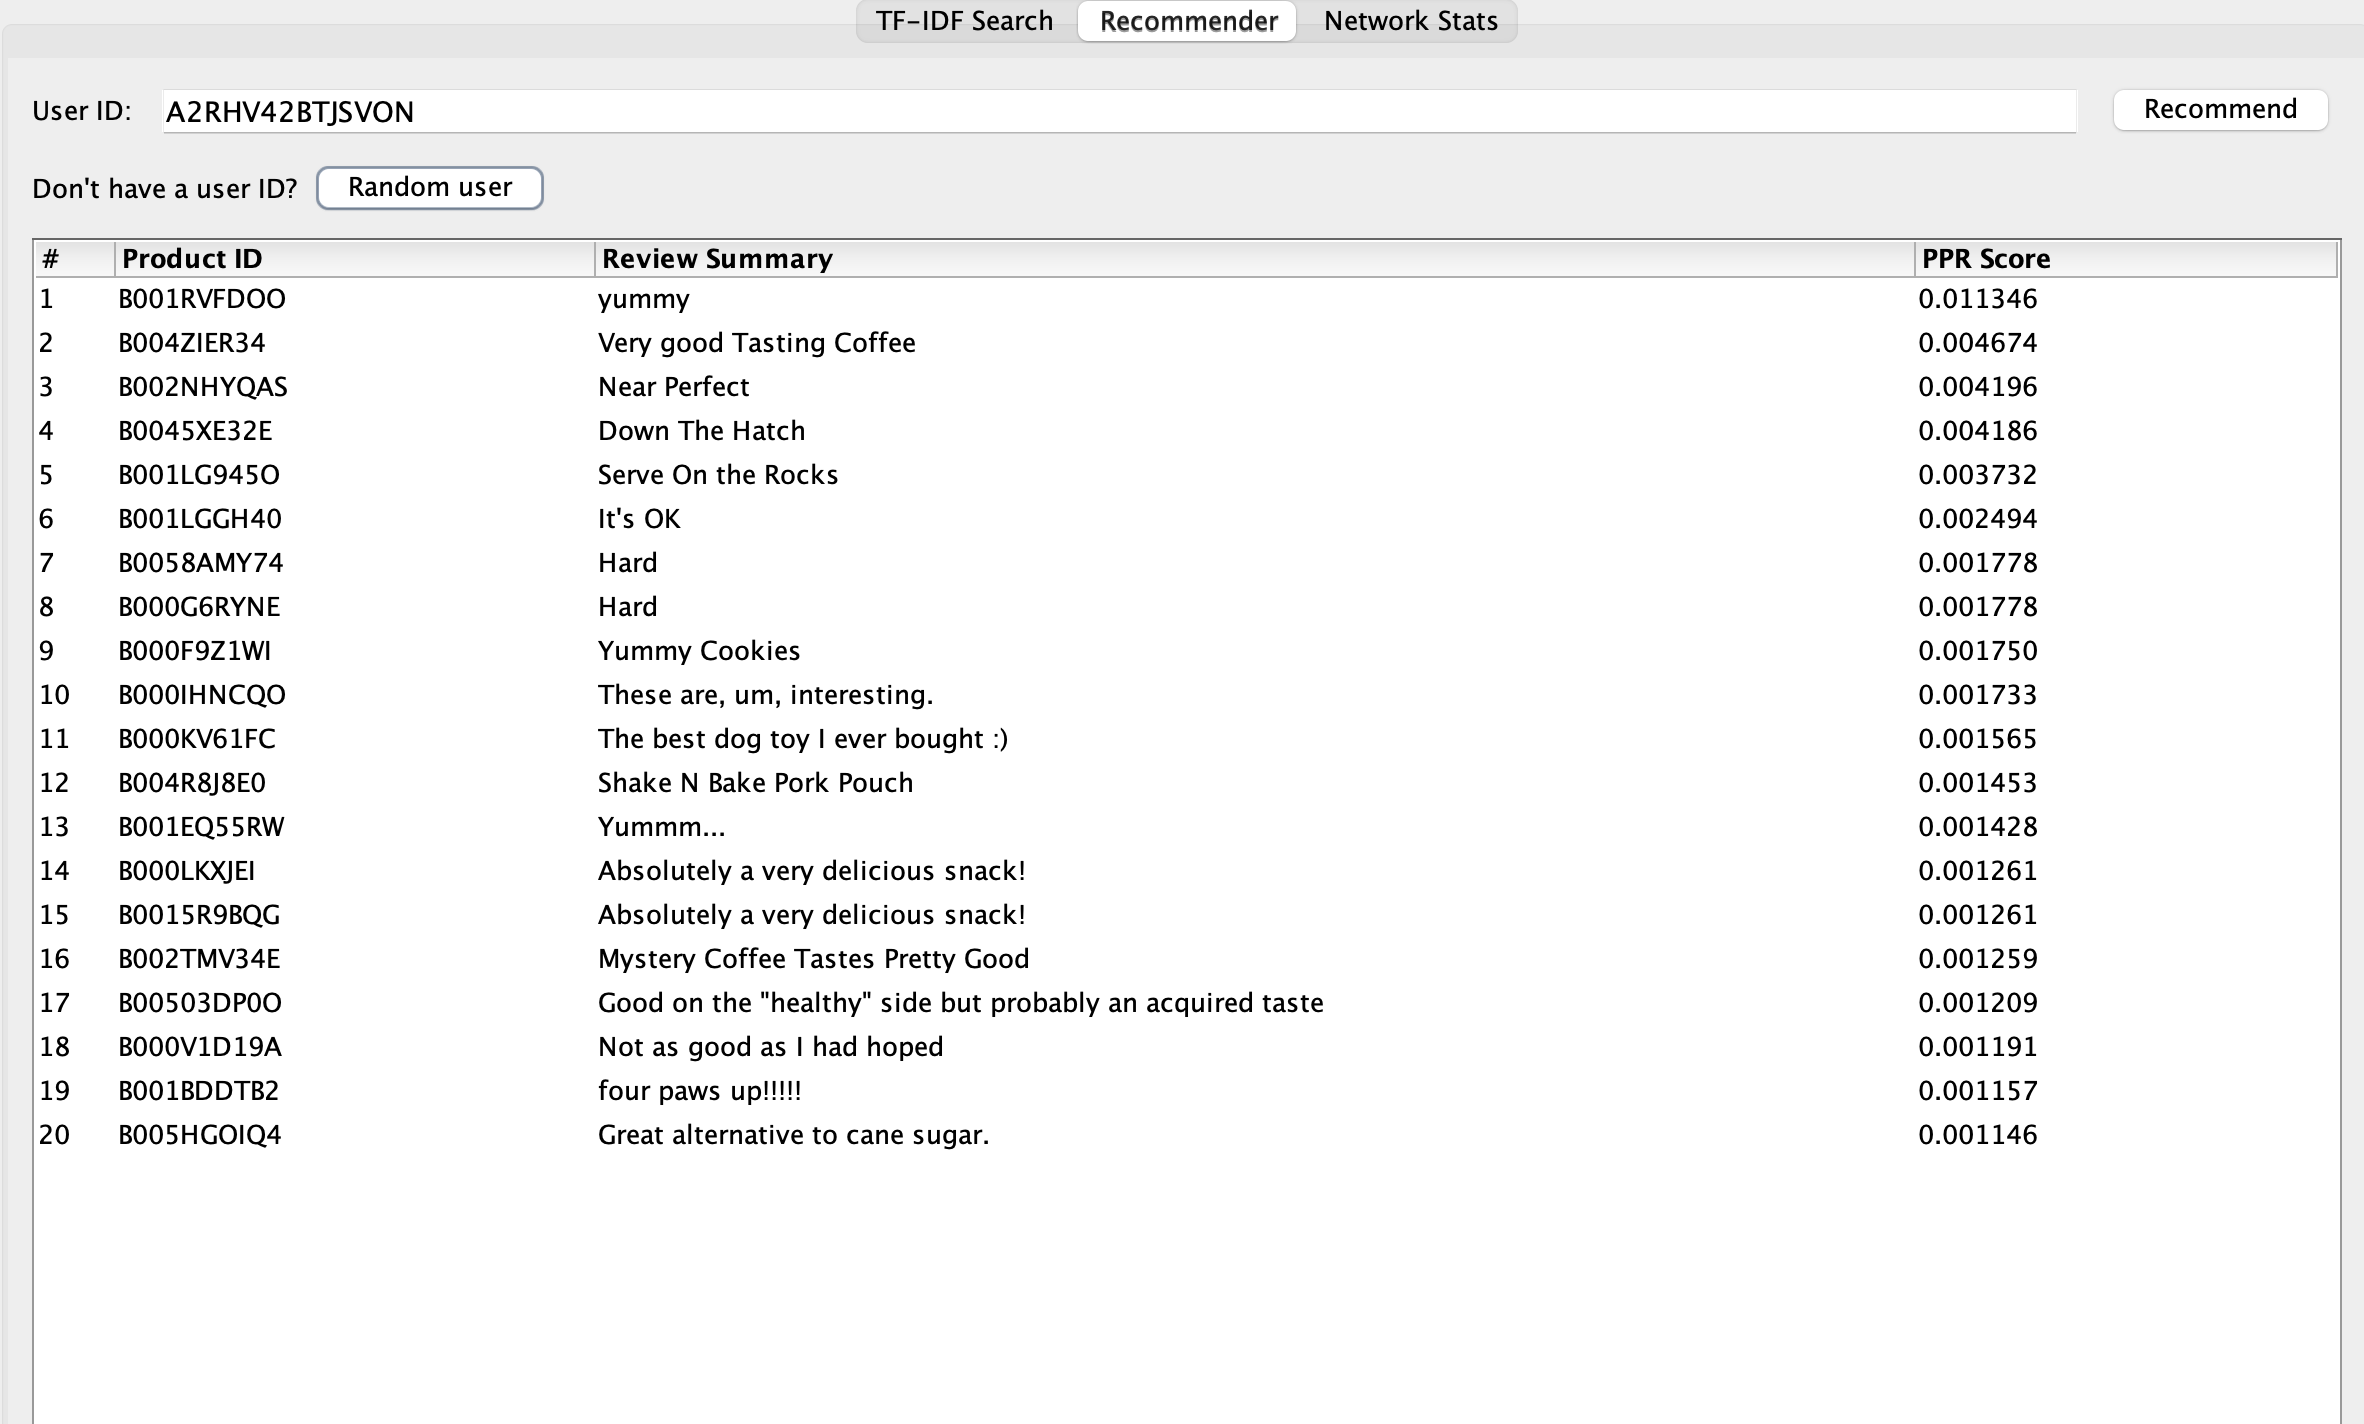
\includegraphics[width=0.9\textwidth]{imgs/recommender-results.png}
\end{figure}

\subsection*{Tab 3: Network Stats}
This tab displays a statistical summary of the bipartite review graph computed by the \texttt{NetworkStats} module.

\begin{figure}[H]
  \centering
  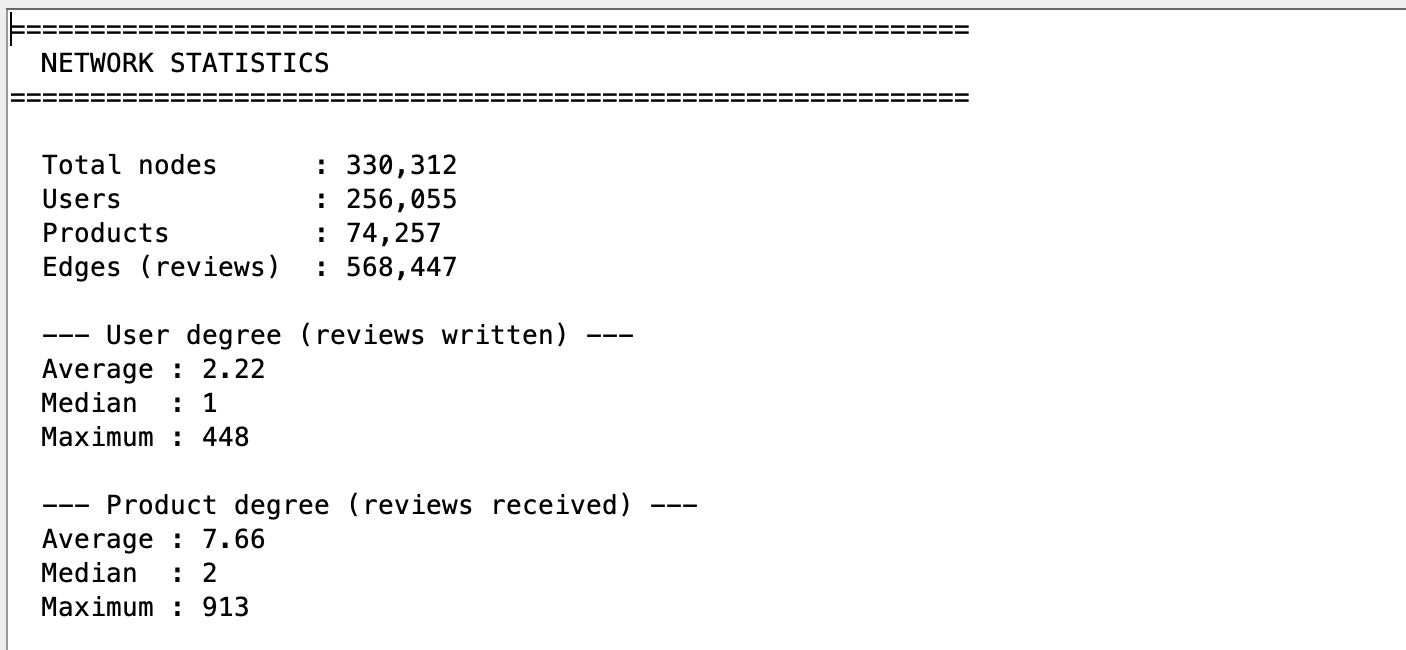
\includegraphics[width=0.48\textwidth]{imgs/network-stats1.png}
  \hfill
  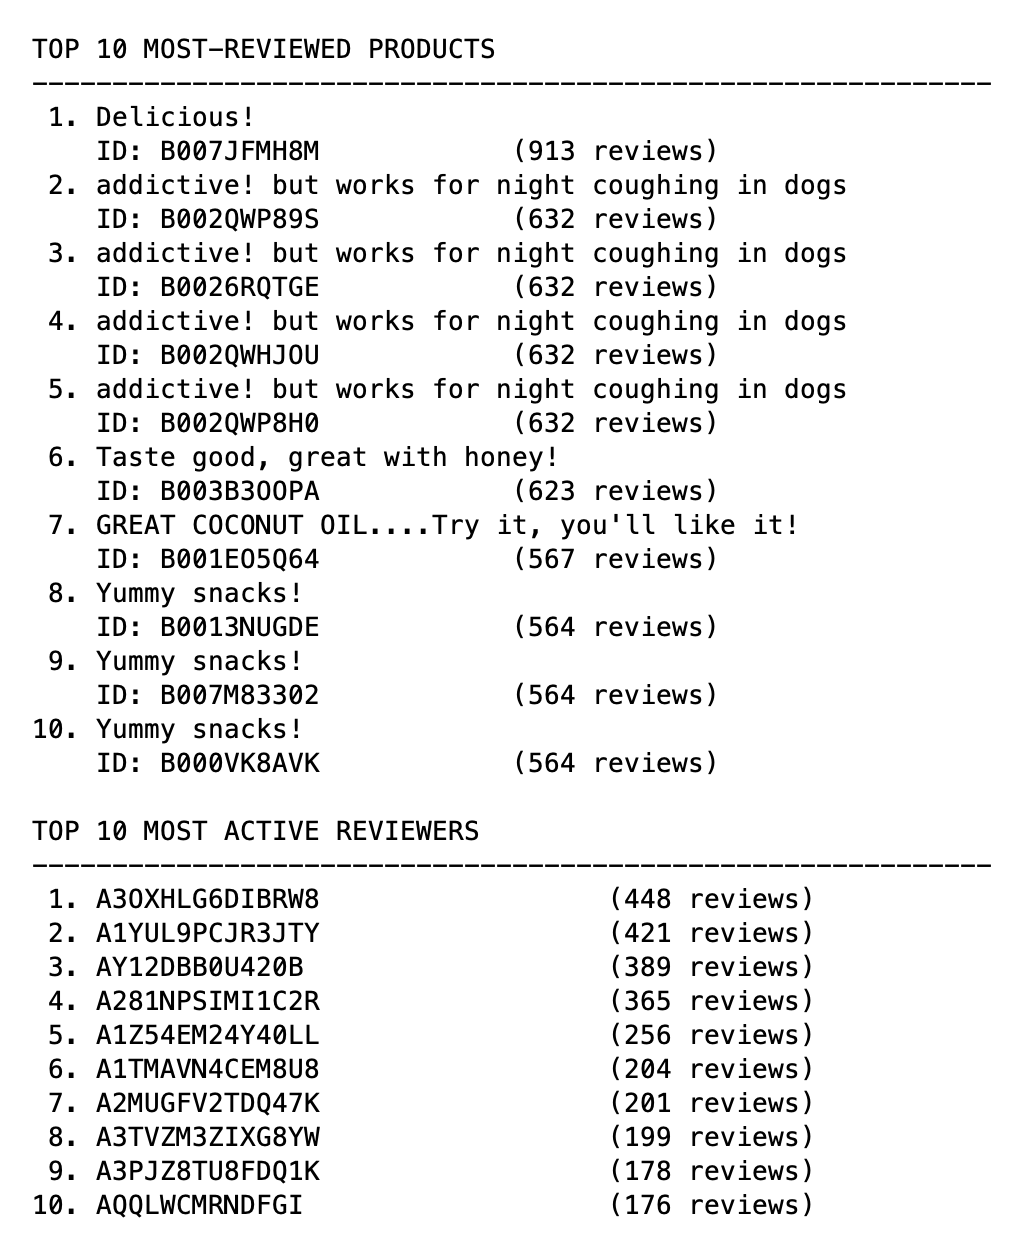
\includegraphics[width=0.48\textwidth]{imgs/network-stats2.png}
  \caption{Network Stats tab showing graph summary and top reviewers/products.}
\end{figure}

Information shown: total node count (broken down into users and products), total edge count, user and product degree statistics (average, median, max), top 10 most-reviewed products, and top 10 most active reviewers. Stats are computed in a background thread when the tab is first opened.

\subsection*{Explanation of Course Concepts}

\subsubsection*{Bipartite Graph}

The application models the review data as a bipartite graph where every reviewer is one kind of node and every product is the other. Edges only connect users to products via undirected edges. Each review becomes a weighted edge, where the weight is the star rating (1--5). Two users who reviewed many of the same products are close in the graph through shared product nodes, even without a direct edge.

\subsubsection*{TF-IDF Document Retrieval}

TF-IDF measures how important a word is to a particular document relative to the full corpus. The engine first builds one document per product by concatenating all its reviews. It then computes Term Frequency (TF), how often each word appears in that document divided by total word count, and Inverse Document Frequency (IDF), which down-weights common words like ``good'' and up-weights rare, distinctive words. The final score is TF $\times$ IDF.

When a user types a query, the system applies the same weighting and returns the products with the highest cosine similarity between the query vector and each product vector.

\subsubsection*{Personalized PageRank Recommender}

The recommender uses Personalized PageRank (random walk with restart) to find products a user is likely to enjoy. It first identifies seed products --- those the user rated 4 or 5 stars --- weighted by rating and normalized to sum to 1. If no 4+ star reviews exist, all reviewed products are used as seeds.

Scores propagate through the graph using the update rule:
\[
PR(v) = (1 - \alpha) \sum_{u \in N(v)} \frac{w(u,v)}{\sum_{z \in N(u)} w(u,z)} \cdot PR(u) + \alpha \cdot s(v)
\]
Here $N(v)$ is the set of neighbors of $v$, $w(u,v)$ is the star rating on the edge between $u$ and $v$, $s(v)$ is the seed score (0 for non-seeds), and $\alpha = 0.15$ is the restart probability. After each iteration the scores are normalized to sum to 1. The algorithm iterates until convergence, i.e.\ until $\sum_{v} |PR_{t+1}(v) - PR_t(v)| < \epsilon$.

Finally, the algorithm removes products the user has already reviewed and returns the remaining products ranked by score.

\end{document}